\documentclass[10pt,a4paper]{article}
\usepackage[utf8]{inputenc}
\usepackage{amsmath}
\usepackage{amsfonts}
\usepackage{amssymb}
\usepackage{titling}
\newcommand{\subtitle}[1]{%
  \posttitle{%
    \par\end{center}
    \begin{center}\large#1\end{center}
    \vskip0.5em}%
}

\usepackage{mathpazo} % Use the Palatino font
\usepackage{graphicx} % Required for including pictures
\usepackage{caption}    % Required for figures side by side
\usepackage{subcaption} % Required for figures side by side

\usepackage{indentfirst} % indentation in first paragraph too
\linespread{1.05} % Change line spacing here, Palatino benefits from a slight increase by default
\usepackage{parskip} % increase parskip to decent amount

\usepackage{titling}              % Get rid of white space on top of document title (generated by \maketitle)
\setlength{\droptitle}{-100pt}

\renewcommand{\thesection}{Exercise \arabic{section}: \hspace{-15pt}}
\renewcommand{\thesubsection}{}

\usepackage{color}
\usepackage{textcomp} % para apostrofe

\usepackage{framed} % para cajetillas en las figuras
\usepackage[table]{xcolor}
\begin{document}

\title{\textbf{Structural Bioinformatics Final Exam}}
\subtitle{RNA part report}
\date{\today}
\author{Antonio Ortega Jiménez}

\maketitle


\section{RNAfold prediction on seq1}

\small{\texttt{AUCAGUUCUAGCAGGAGCUGUACUCAGAGACUCGGGAAAUUUUCCCGGAAUUUUACCCGGGUUUUUACGU}} \\
\small{\texttt{..(((((((....))))))).....(((((((((((.((..(((...)))..)).)))))))))))....}}

\textbf{a)} The obtained Minimum Free Energy (MFE) secondary structure consists of a multiloop with two closed components. The left arm contains a hairpin, whereas the right arm contains another hairpin with a couple of internal loops. The centroid version discards these internal loops and instead shows a simple hairpin with a huge loop. This is due to the low probability exhibited by the base pairs in the terminal region of the hairpin \cite{gorodkin}.

\textbf{b)} RNAfold predicts 18 base pairs with a probability higher than 0.8.


\begin{figure}[!h]
    \centering
    \begin{subfigure}[b]{0.4\textwidth}
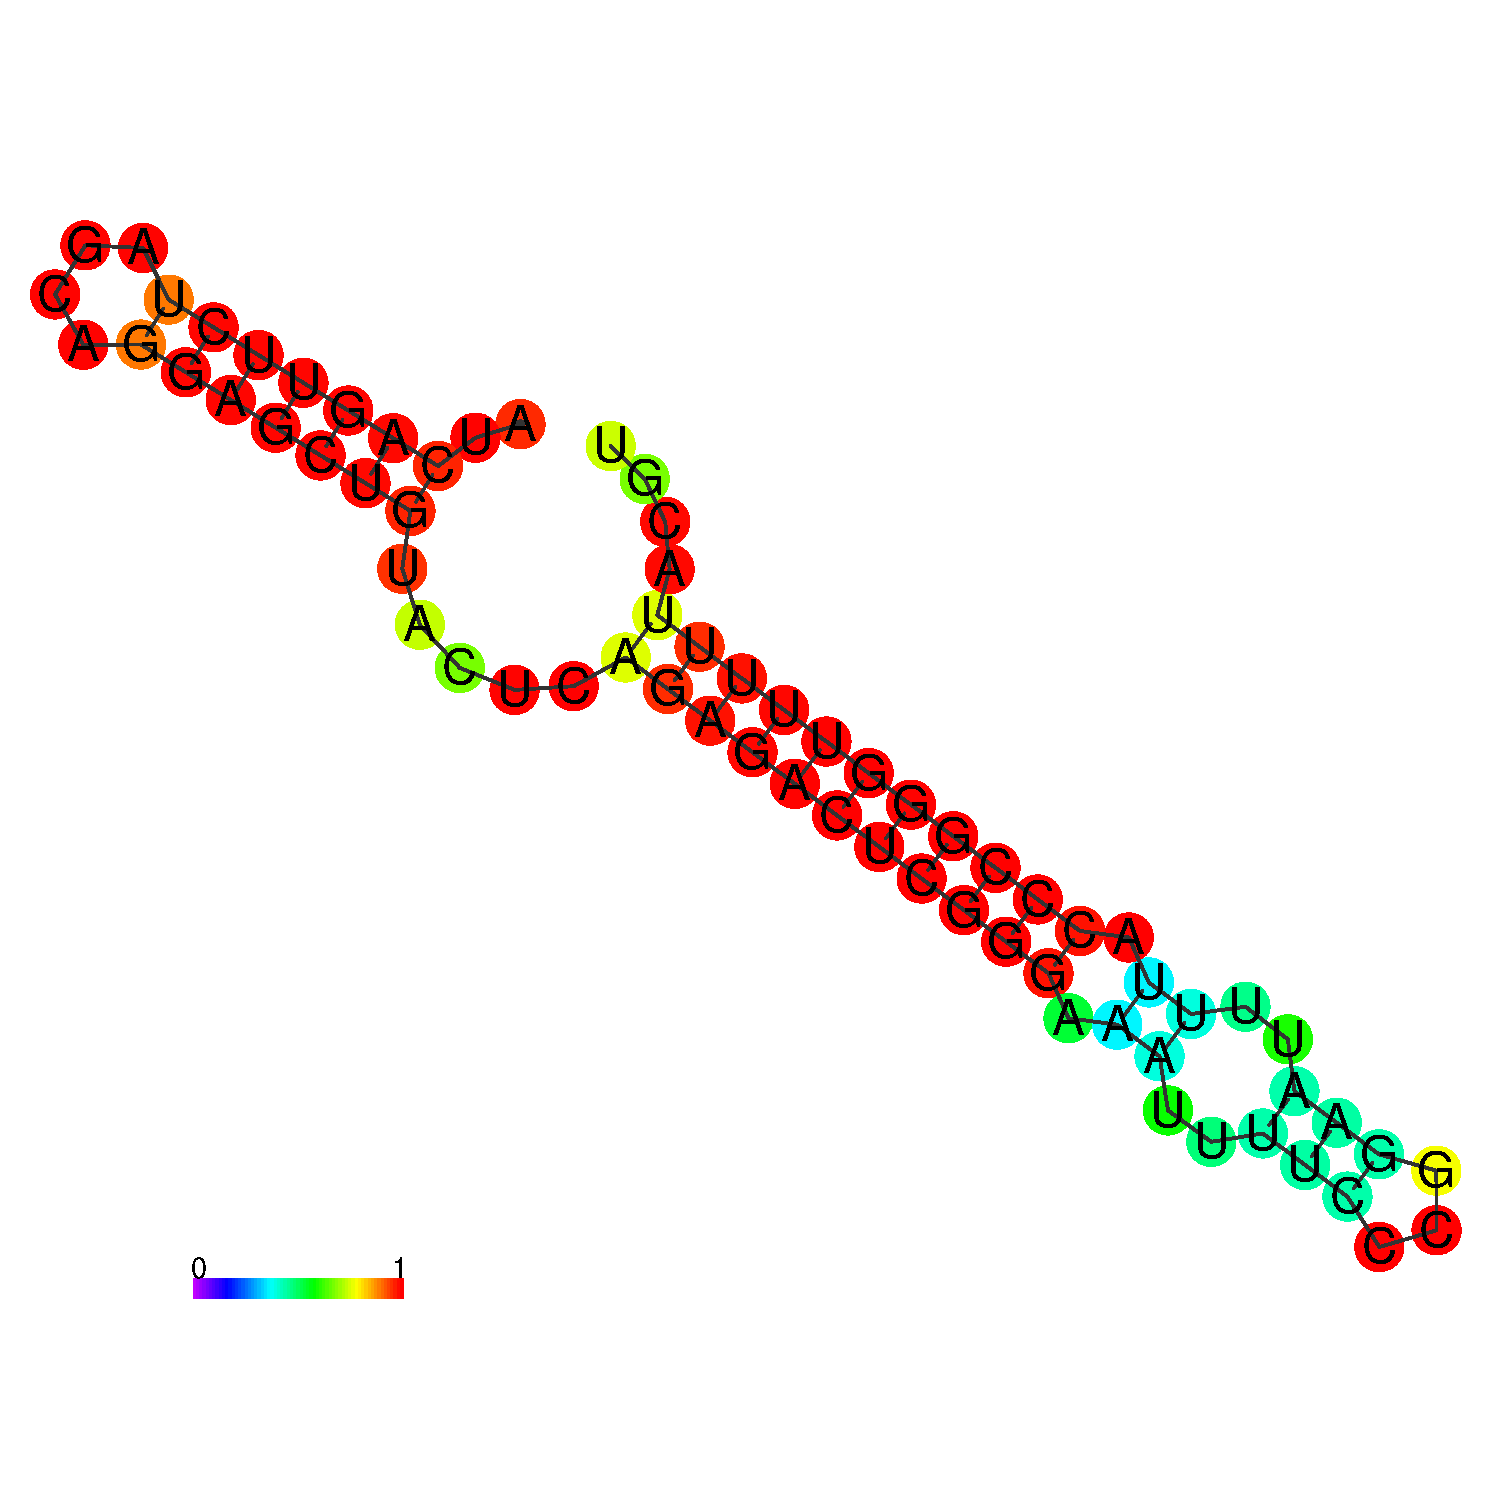
\includegraphics[width = \textwidth]{figures/sequence1_pp.eps}
        \caption{Minimum Free Energy (MFE) structure}
        \label{fig:MFE_1}
    \end{subfigure}
~
\begin{subfigure}[b]{0.4\textwidth}
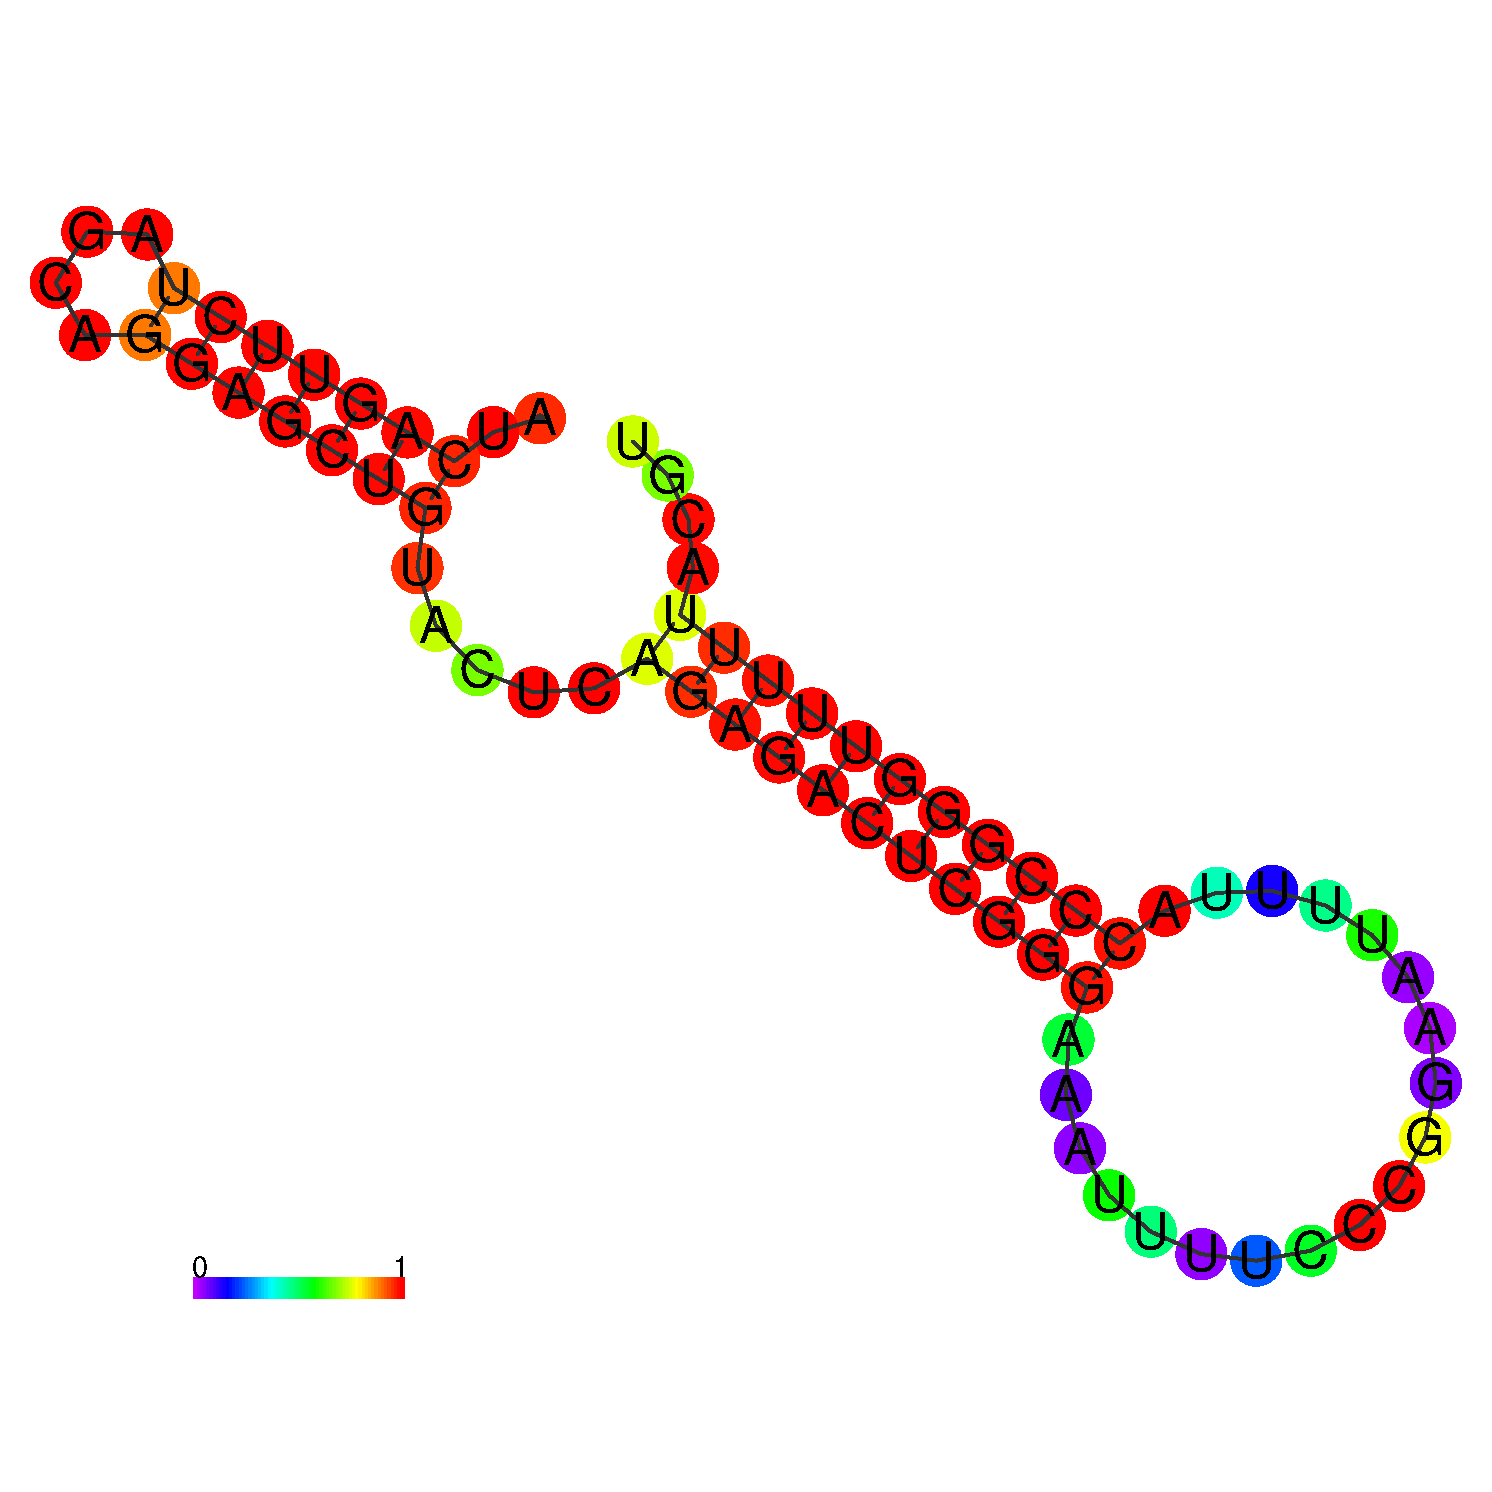
\includegraphics[width = \textwidth]{figures/sequence1_centroid_pp}
        \caption{Centroid structure}
        \label{fig:CNT_1}
    \end{subfigure}
\caption{Structures predicted by RNAFold for the query sequence. The color code shows base pair probabilities.}
\end{figure}


\section{RNAfold prediction on seq2}


\small{\texttt{AUCGGUUCCAGCAGGAACUGUACUCGGGGGCUCGGGAAACCCUCCCGGGGUUUUACCCGGGUUUUUACGU}} \\
\texttt{..(((((((....))))))).(((((((..(((((((.....)))))))......)))))))........}

\textbf{a)} \textit{A priori}, this sequence has a similar structure. Base pairs are distributed differently in the right arm, and this has triggered an increase in the hairpin stability. This can be easily noticed:

\begin{itemize}

\item The centroid structure now includes the hairpin, because there are more structures in the ensemble that now feature the same hairpin.

\item Instead of a highly stable duplex and a highly unstable loop, stability is uniformly distributed across the whole hairpin (see second bulge in right violin from figure \ref{fig:violin}). This enables the formation of the most interior bonds in the duplex, right before the hairpin\textquotesingle s loop, which therefore grows smaller.

\item Thermodynamical ensemble prediction parameters show that the structural diversity is reduced and the frequency of the MFE structure increases.

\end{itemize}

\textbf{b)} RNAfold predicts 20 base pairs with a probability higher than 0.8.

\begin{figure}[!h]
    \centering
    \begin{subfigure}[b]{0.4\textwidth}
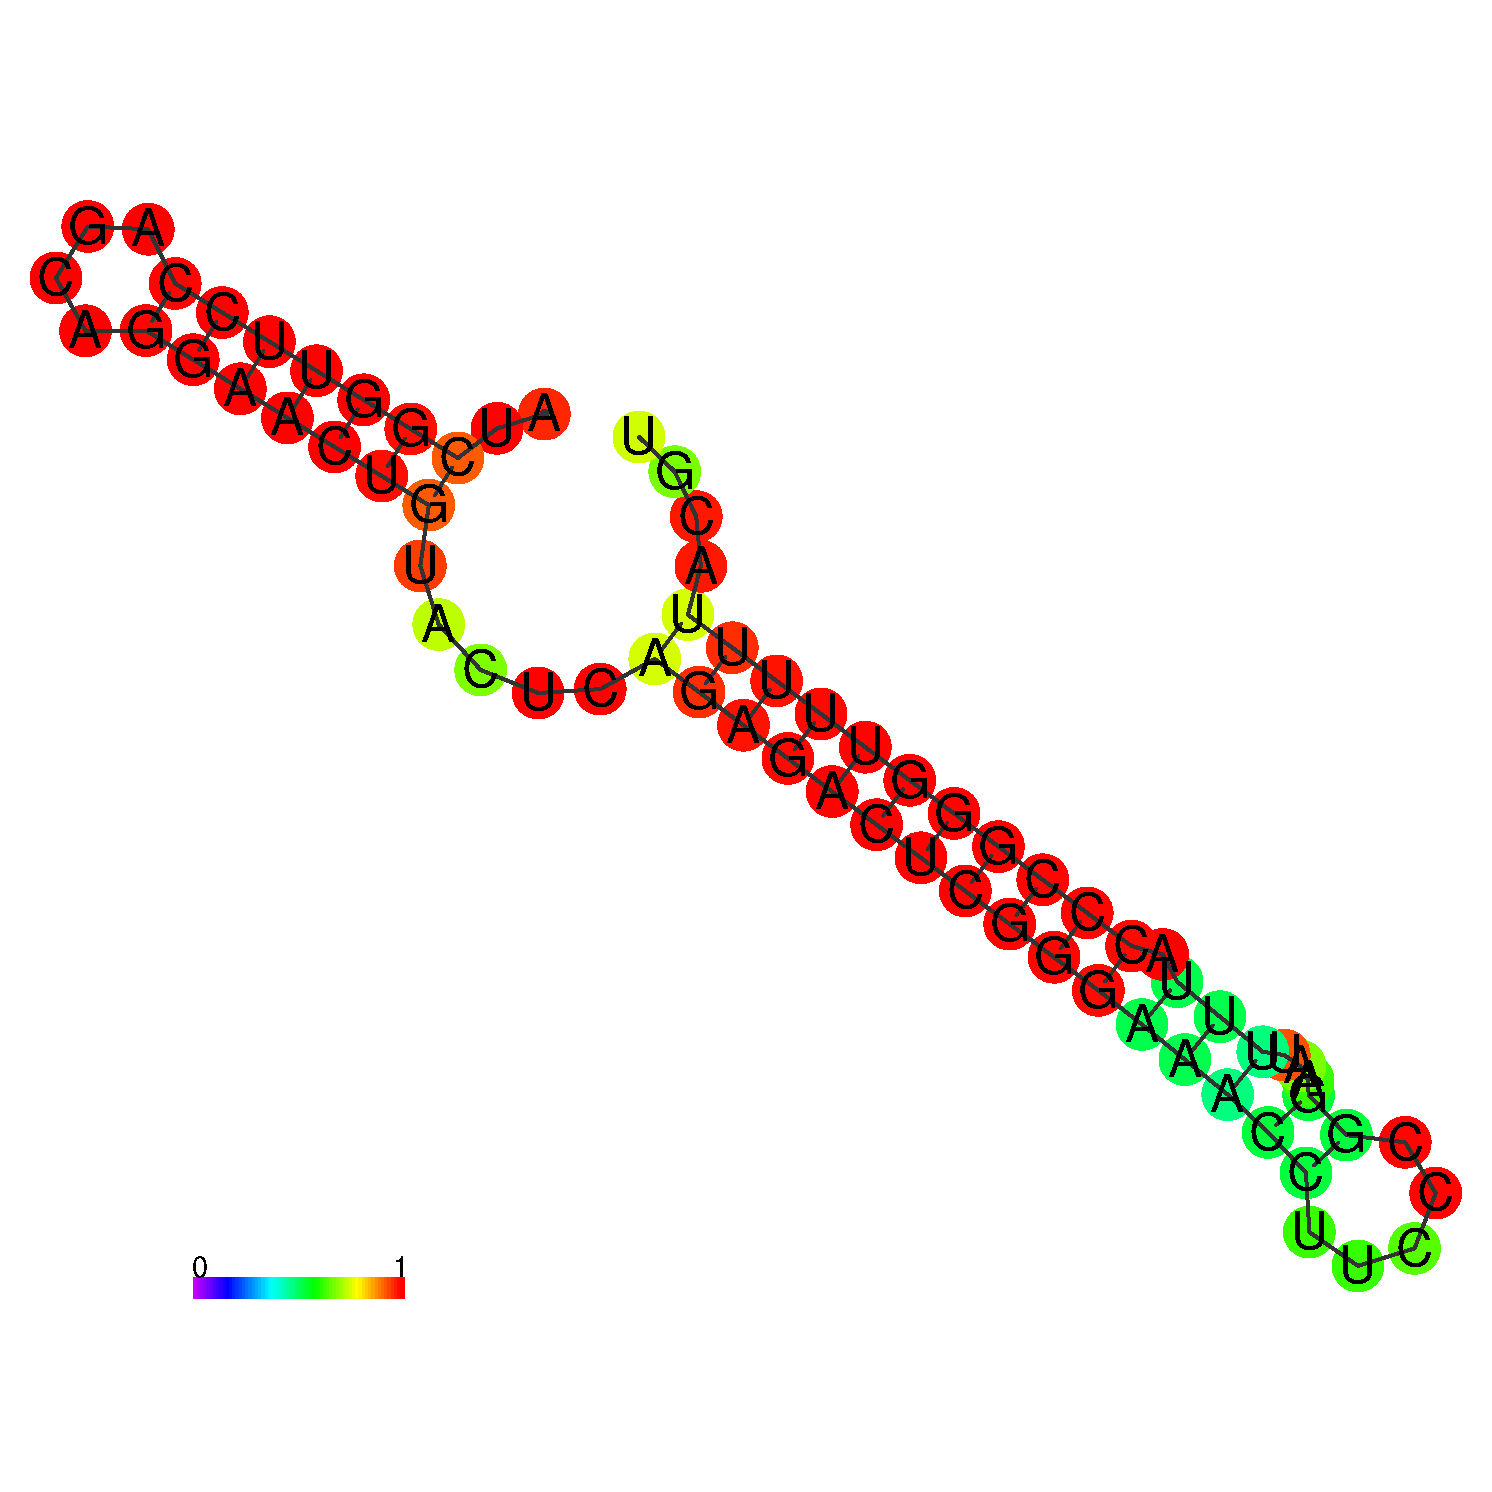
\includegraphics[width = \textwidth]{figures/sequence2_pp.eps}
        \caption{Minimum Free Energy (MFE) structure}
        \label{fig:MFE_2}
    \end{subfigure}
~
\begin{subfigure}[b]{0.4\textwidth}
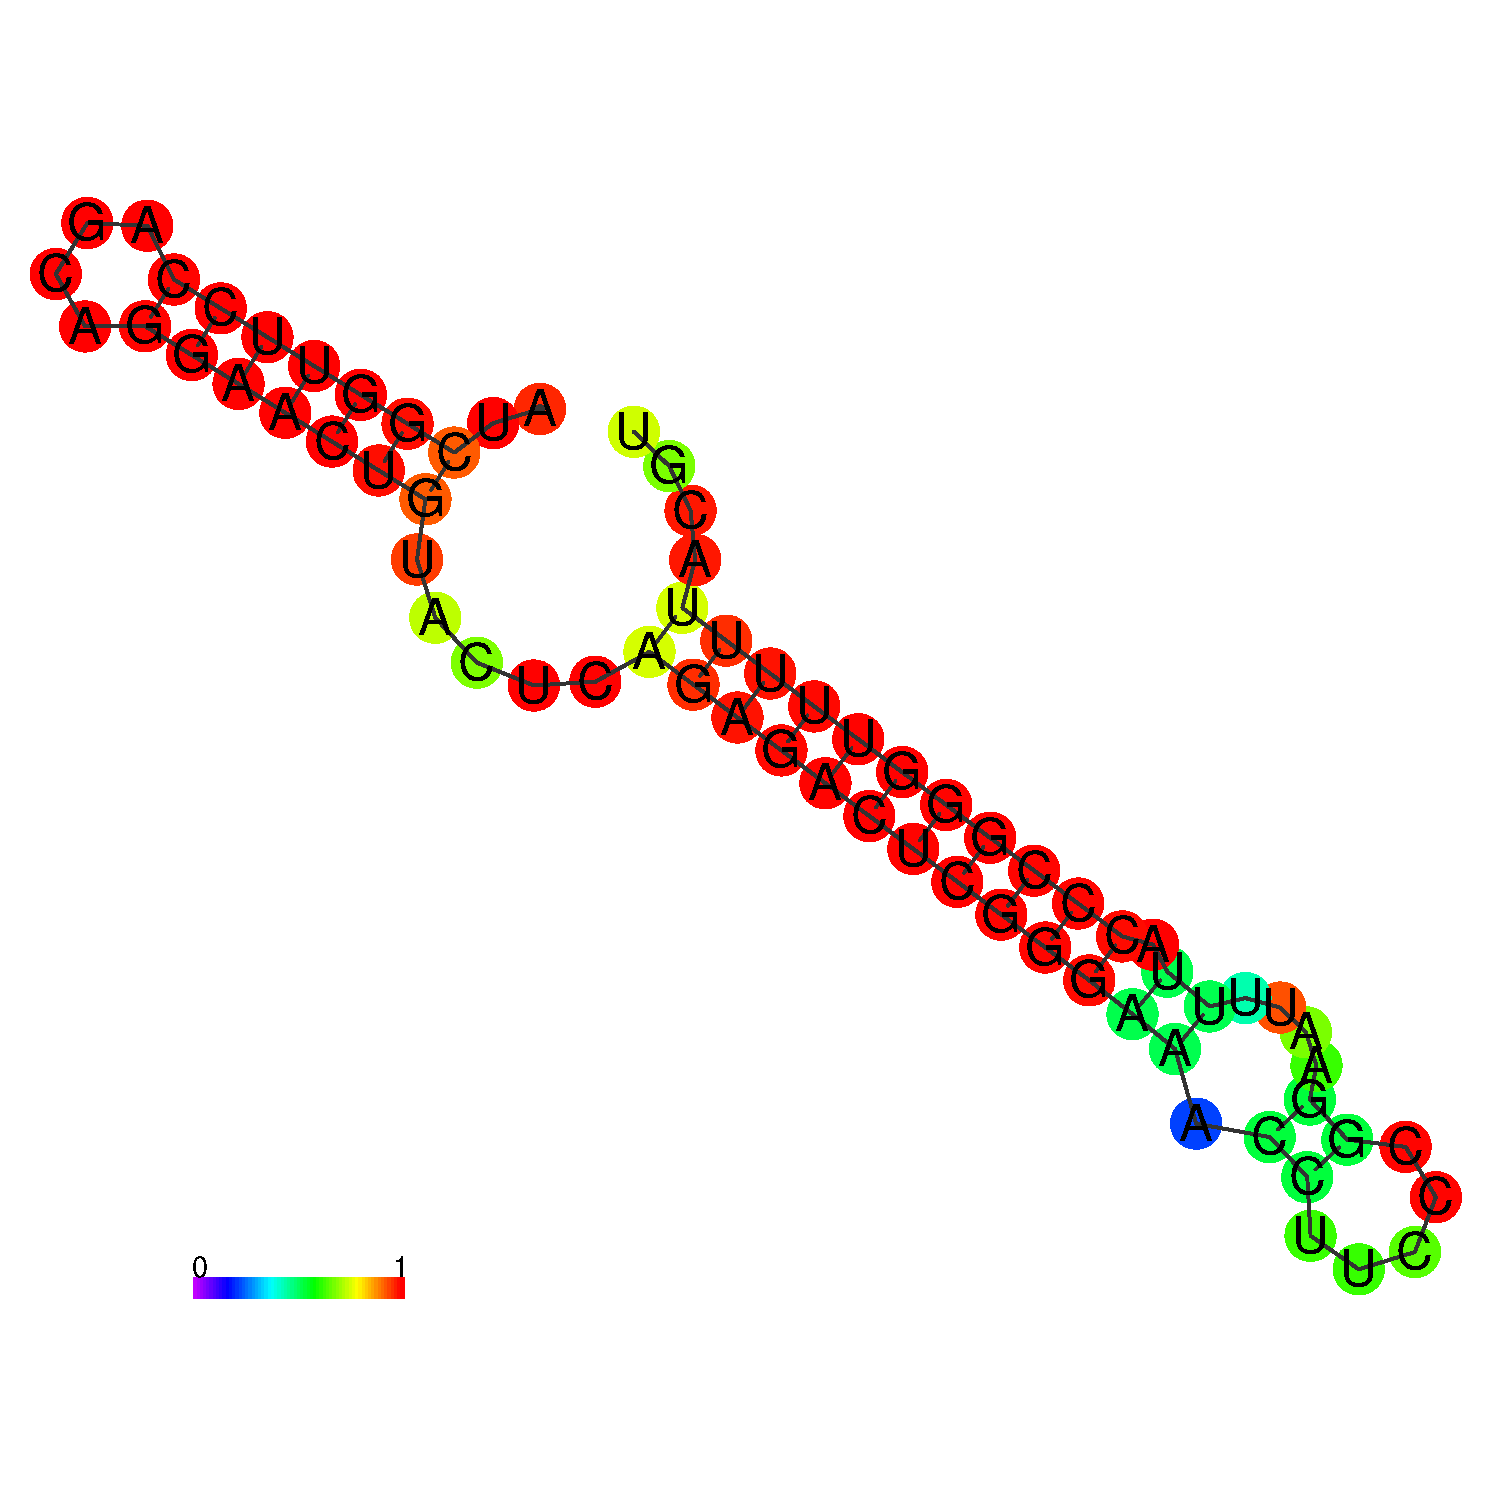
\includegraphics[width = \textwidth]{figures/sequence2_centroid_pp}
        \caption{Centroid structure}
        \label{fig:CNT_2}
    \end{subfigure}
\caption{Structure predicted by RNAFold for the query sequence. The color code shows base pair probabilities.}
\end{figure}

%\subsection{Visualization of base pair probability distributions}

\section{Hamming distance}

Hamming distance between structures is 22, and just 11 at the sequence level.


\section{Base pair distance}

Base pair distance between structures is 30.

\section{Discussion}

Both sequences have a high identity, with a Hamming distance of just 11 at the sequence level. Nevertheless, these differences are not uniformly distributed across the sequence, and thus, they exert different impacts on each arm.

\begin{itemize}

\item In spite of the 3 mutations suffered by the left arm, on positions 3 10 and 18, the structure is not changed. This is due to the consistent nature of these mutations, that preserve the affected base pairs:

\begin{center}

\texttt{A-U $\rightarrow$ G-U} \textbar
\texttt{U-G $\rightarrow$ C-G} \textbar
\texttt{U-G $\rightarrow$ U-A}

\end{center}

The dotplots (figure \ref{fig:dotplot}) support the idea that the left arm has not changed: no significant differences are observed in the left arm area (top left corner), and no alternative structures are observed within the probability space.


\begin{figure}[!h]
    \centering
    \begin{subfigure}[b]{0.25\textwidth}
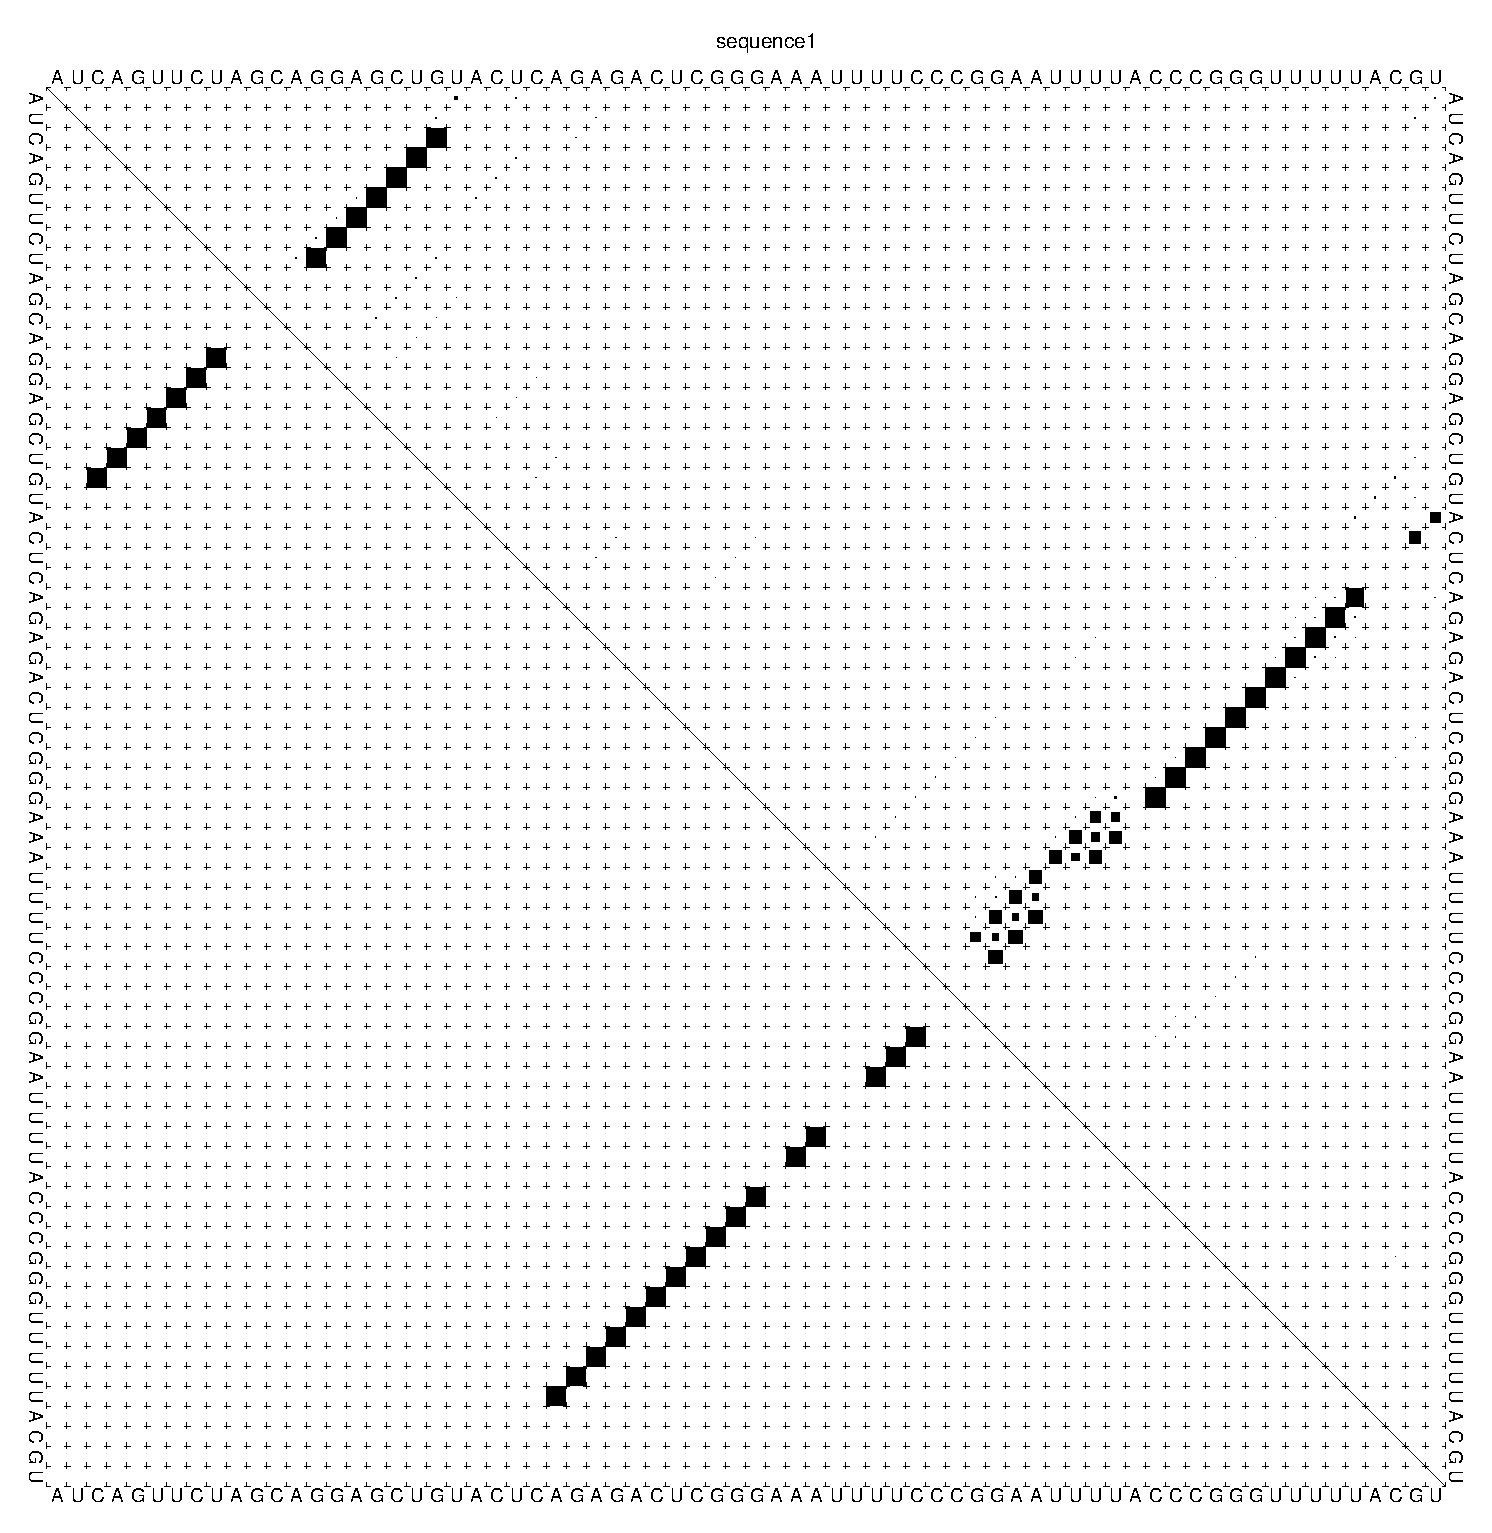
\includegraphics[width = \textwidth]{figures/sequence1_dp.eps}
    \end{subfigure}
~
\begin{subfigure}[b]{0.25\textwidth}
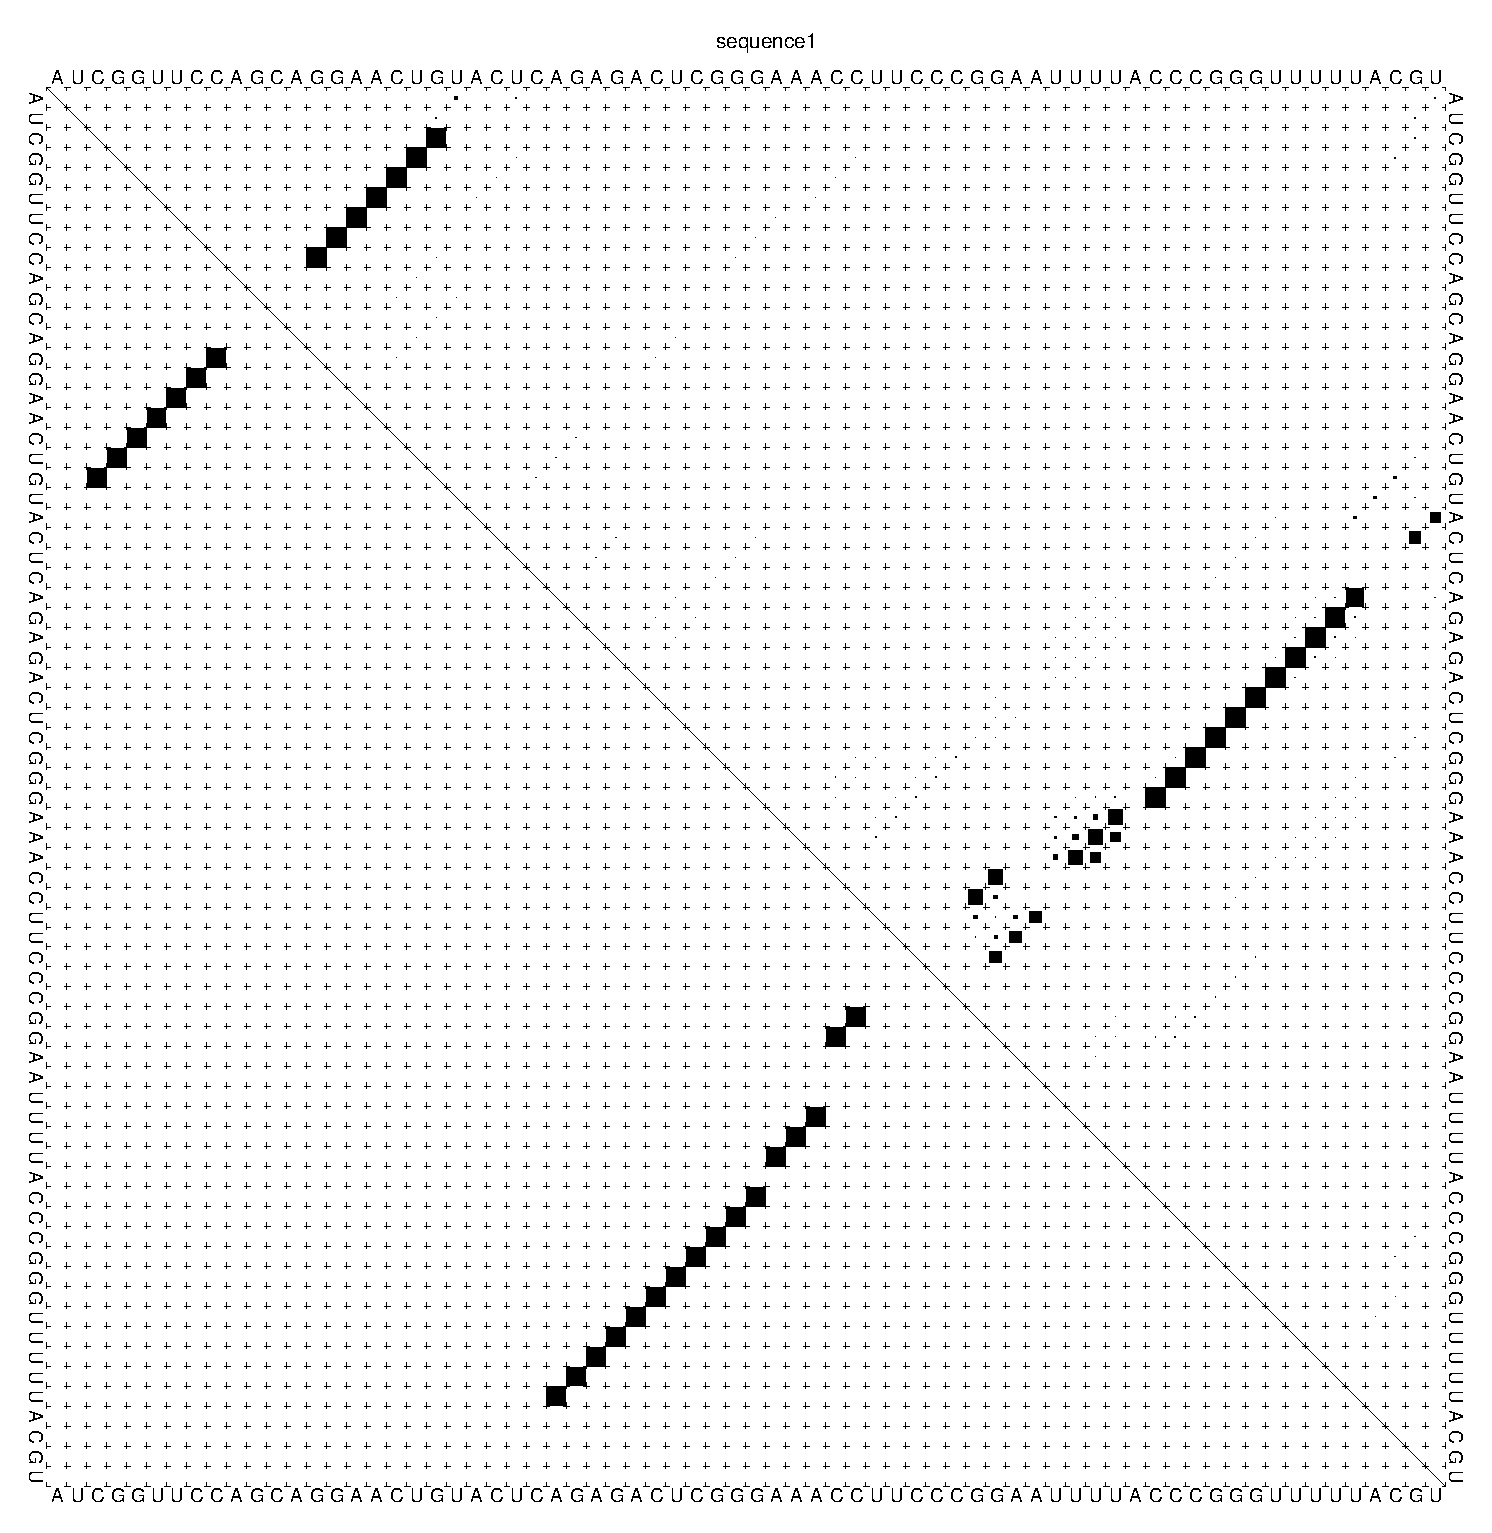
\includegraphics[width = \textwidth]{figures/sequence2_dp.eps}
    \end{subfigure}
    \caption{Base pair probability dot plot for seq1 (left) and seq2 (right)}
\label{fig:dotplot}
\end{figure}


\item The remaining 8 mutations are located on the right arm, and though the structural motif is preserved, its internal organization has changed totally.

\subitem On the one hand, base pairs cluster into 2 blocks of the same length (7 base pairs each, 14 in total), instead of 3 blocks of length 11, 2 and 3 (16 in total). This organization leads to a unique internal loop in the duplex center. Since internal loops and bulges destabilize duplexes, as stated in \cite{} it follows that a reorganization that reduces the number of internal loops is bound to make the structure more stable.

\begin{center}
\footnotesize{\texttt{..(((((((....))))))).....(((((((((((.((..(((...)))..)).)))))))))))....} \\
\texttt{..(((((((....))))))).(((((((..(((((((.....)))))))......)))))))........}}  \\
\end{center}
\hspace*{4.4em} \textcolor{red}{\textbf{left arm}} \hspace*{12em} \textcolor{blue}{\textbf{right arm}}



\subitem On the other hand, this reorganization leads to a redistribution of base pairing probability toward inner regions of the duplex, that become more stable. In other words, in exchange for the loss of 2 base pairs, the remaining ones become more stable and trigger the stabilization of the hairpin\textquotesingle s duplex. As a result, the whole hairpin in the right arm is more probable. This phenomenon can be easily observed in figure \ref{fig:violin}.


\end{itemize}


\begin{figure}[!h]
\centering
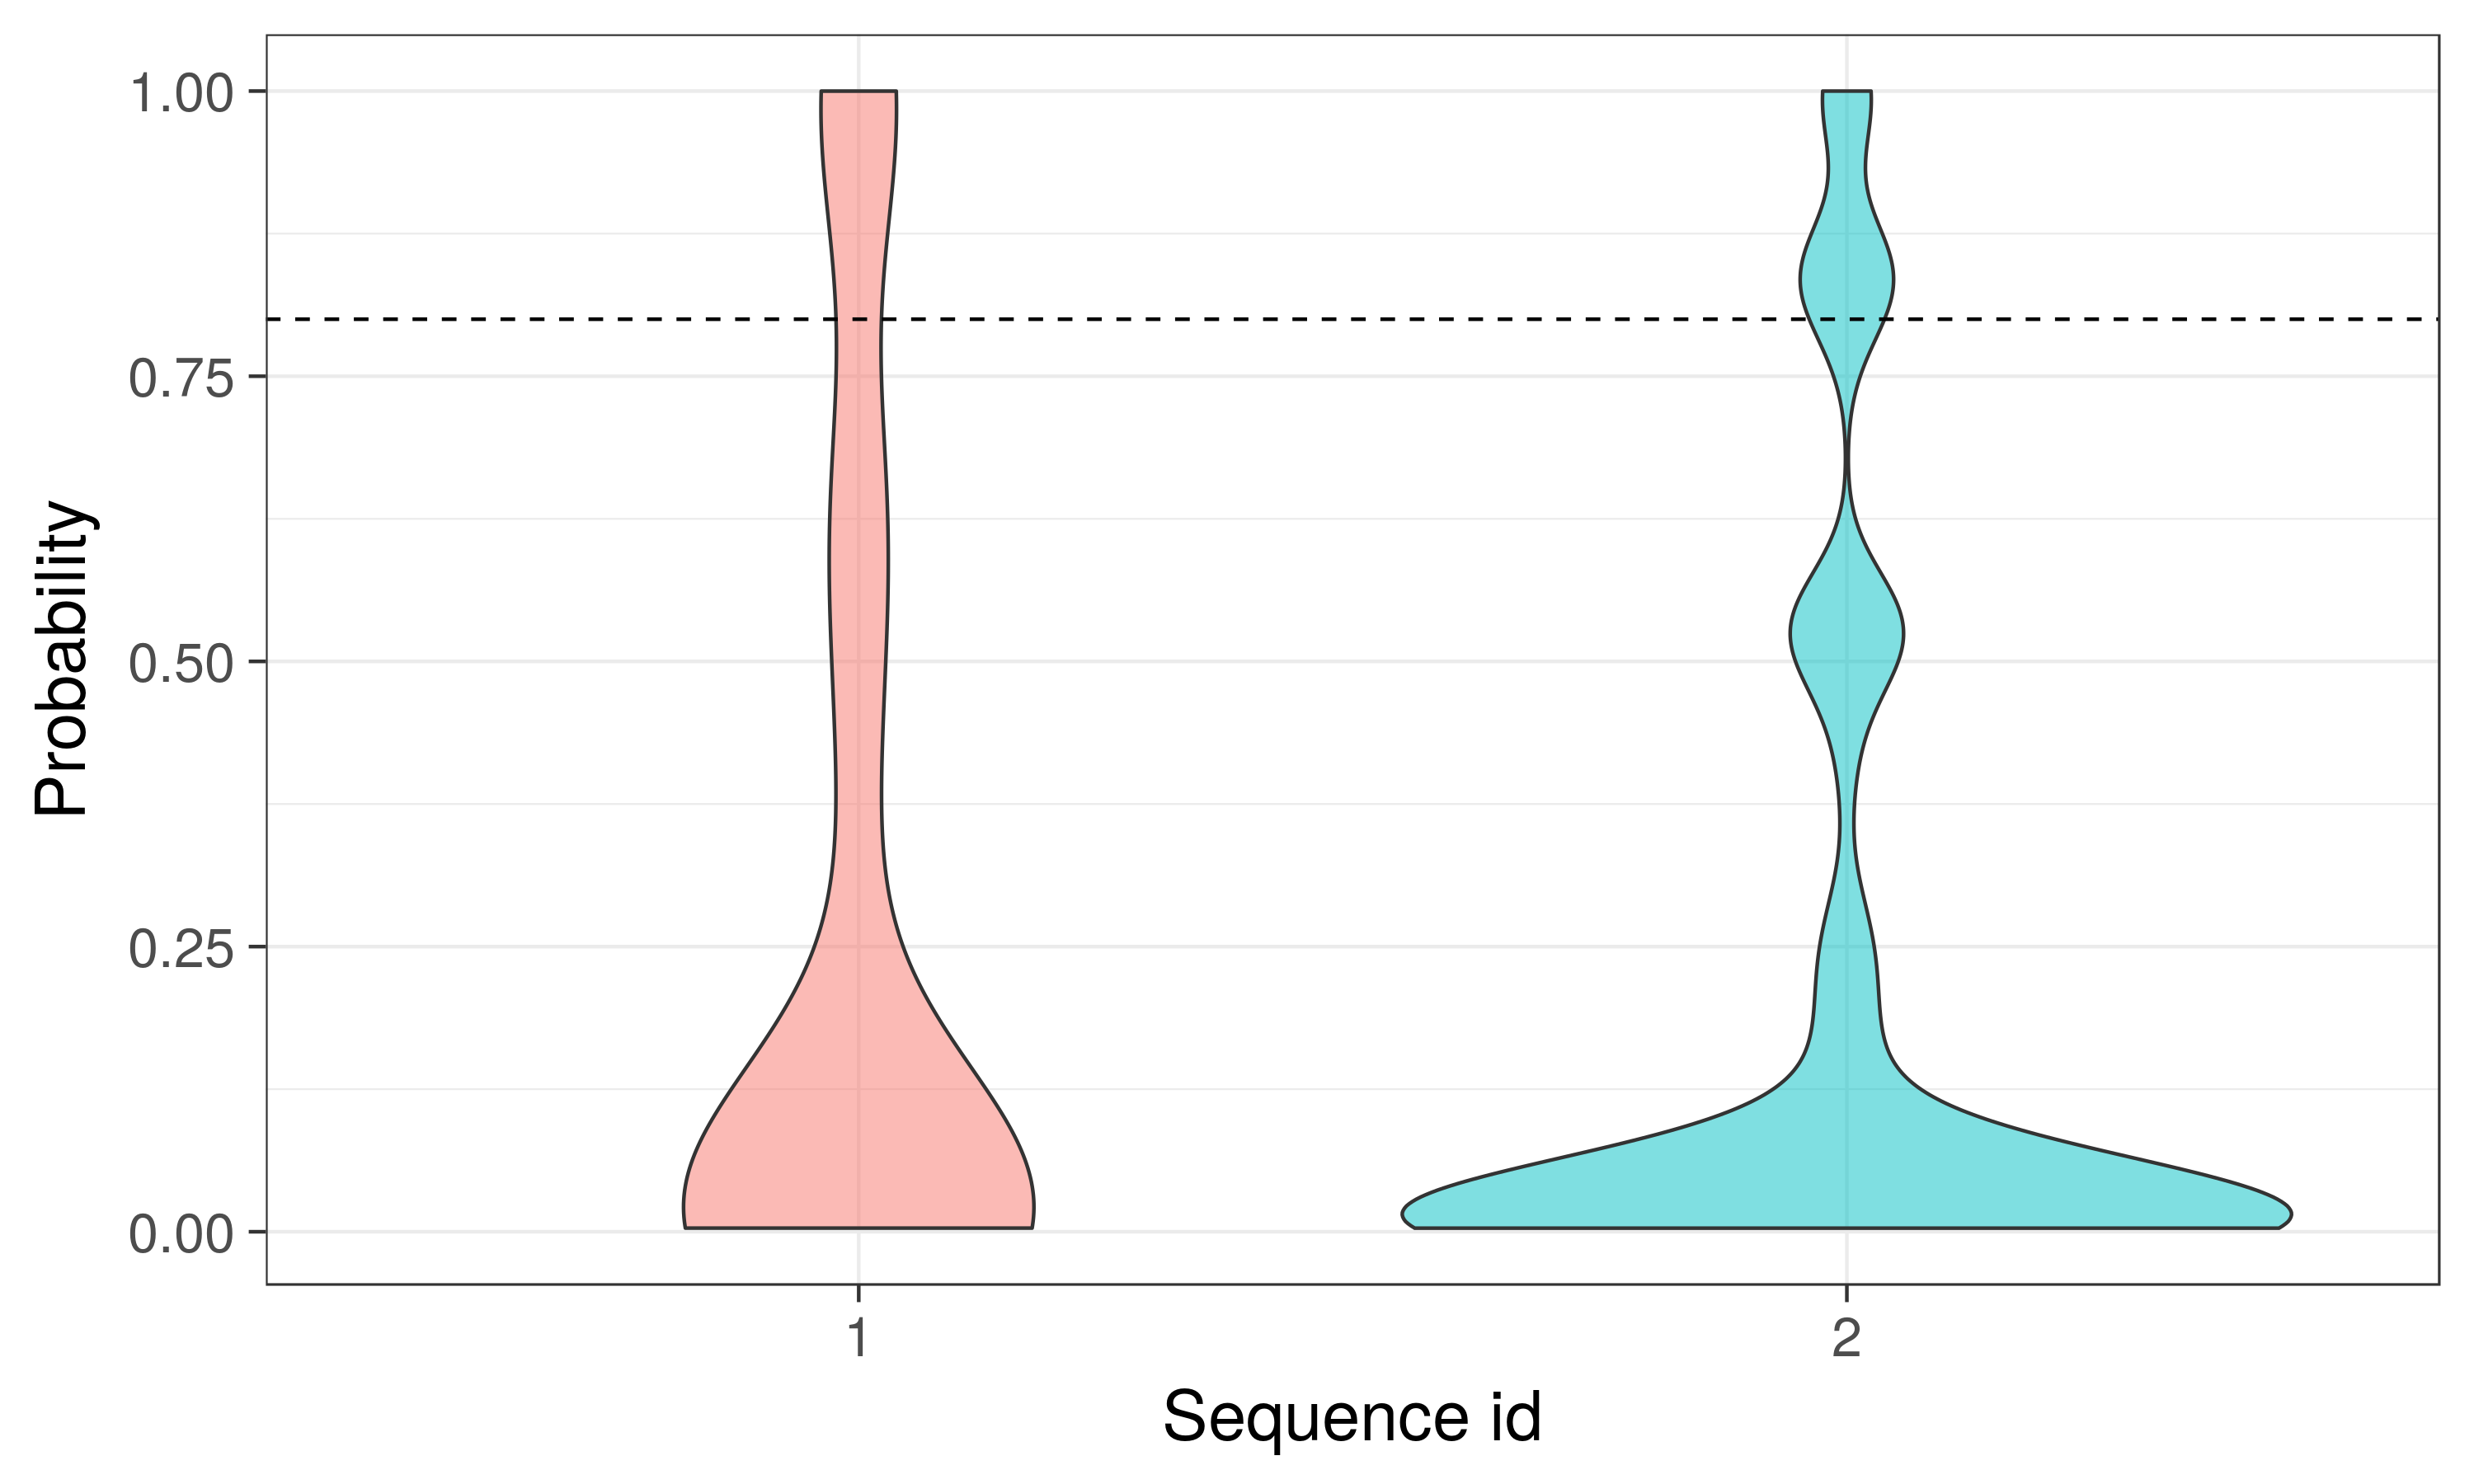
\includegraphics[width = 0.6\textwidth]{figures/violin.png}
\caption{Violin plot showing the base pair probabilities distribution. In sequence 1, we observe a linear gradient of base pair probabilities. In sequence 2, the gradient is broken, and instead a central probability value, around 0.5, becomes very frequent. This represents the uniform base pair probability value newly acquired across the whole right arm.}
\label{fig:violin}
\end{figure}




\section{RNAalifold}

The sequence returned by the RNAalifold server when queried with the proposed alignment of seq1 and seq2 is exactly the same as seq2. Indeed, both the Hamming distance and the base pair distance between the consensus and seq2 are 0.



\begin{figure}[!h]
\begin{framed}

\textbf{Consensus returned by RNAalifold}

\small{\texttt{AUCGGUUCCAGCAGGAACUGUACUCGGGGGCUCGGGAAACCCUCCCGGGGUUUUACCCGGGUUUUUACGU}} \\
\texttt{..(((((((....))))))).(((((((..(((((((.....)))))))......)))))))........}

\centering    
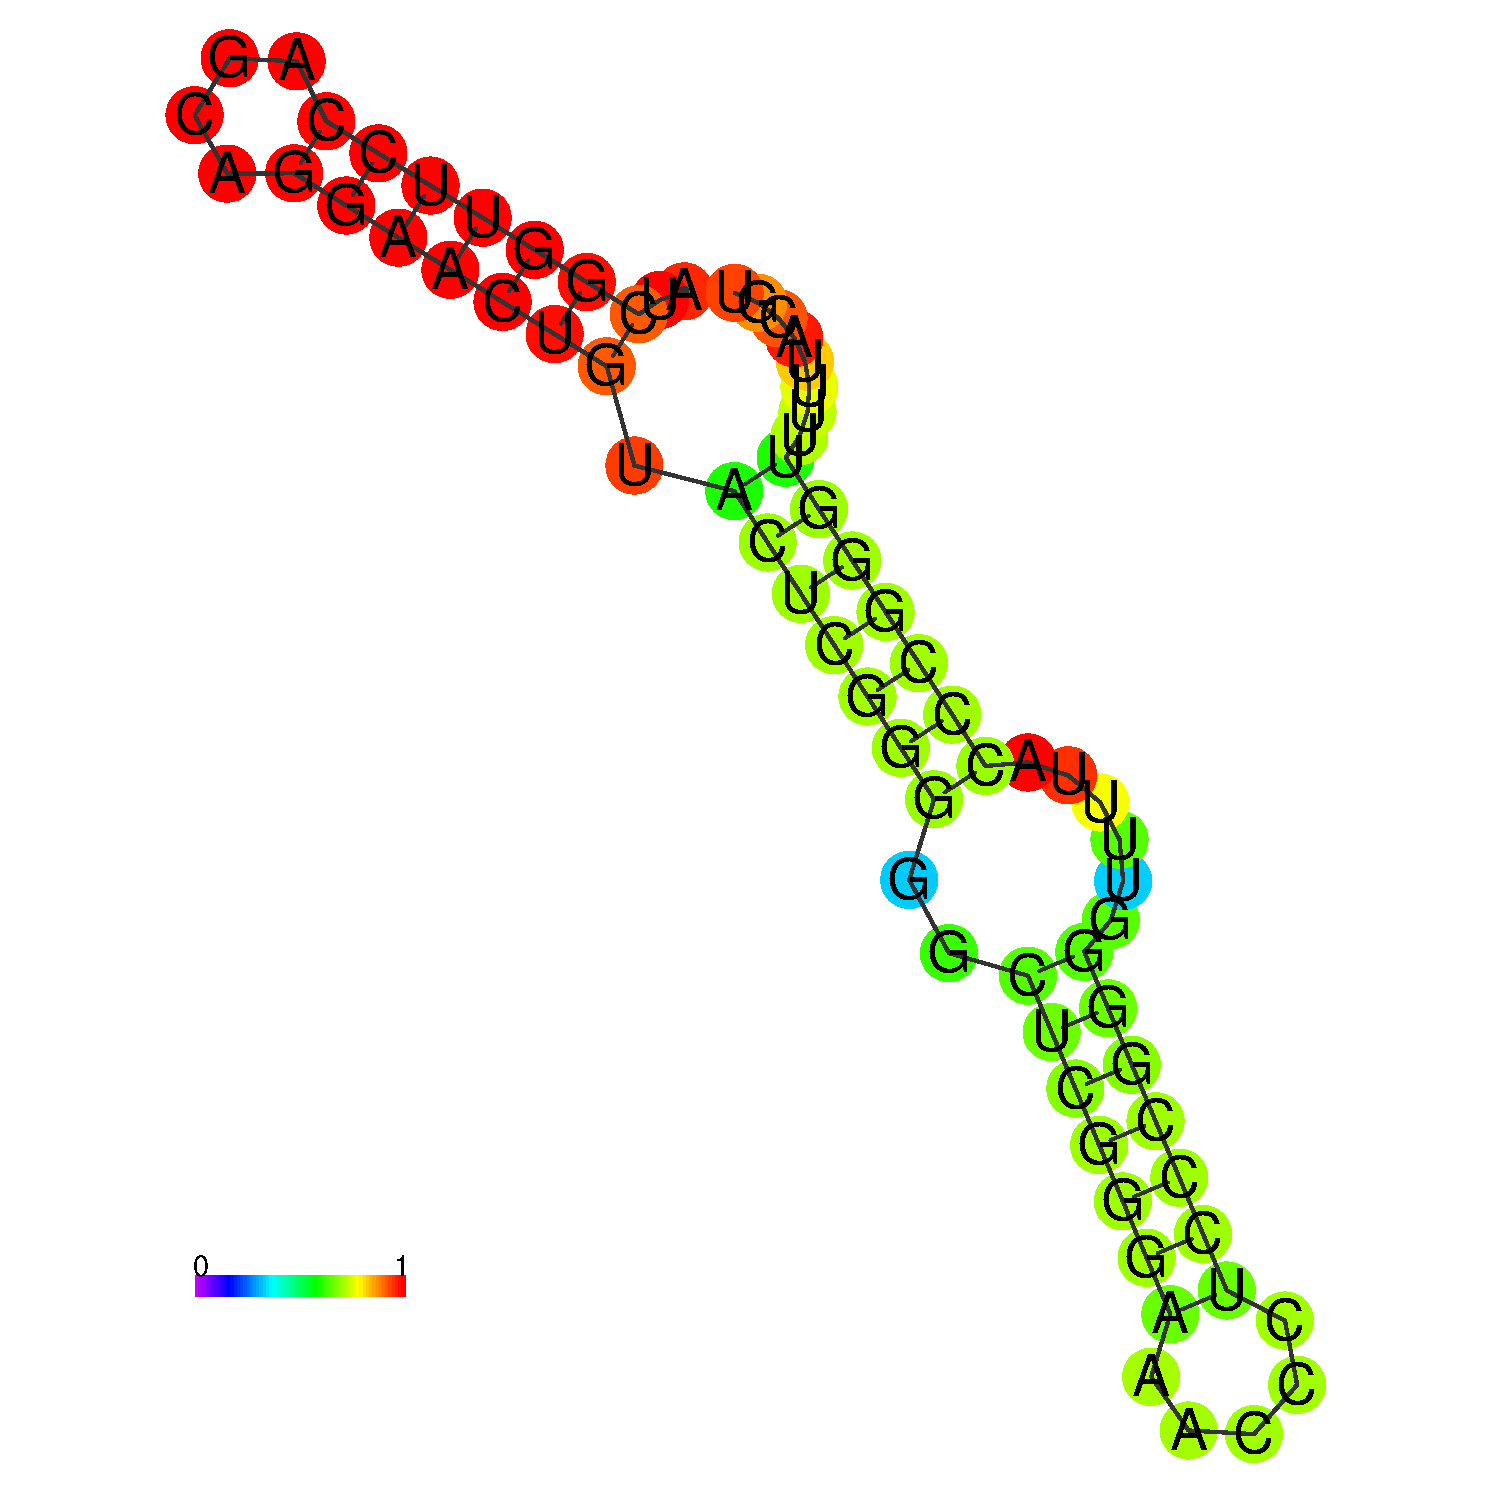
\includegraphics[width = 0.5\textwidth]{figures/alirna_pp.eps}
\caption{Consensus structure predicted by RNAalifold for the queried alignment of seq1 and seq2. The color code shows base pair probabilities.}
\label{fig:ali}

\end{framed}
\end{figure}



\begin{table}
\begin{center}
  \rowcolors{2}{red!25}{white}
  \begin{tabular}{r cc}
    \rowcolor{red!50}
     & Hamming & Base pair \\
seq1 &  22 & 30 \\ seq2 & 0 & 0
  \end{tabular}
  \caption{Hamming distance and base pair distance at the structure level between each individual sequence and the RNAalifold consensus.}
\end{center}
\end{table}


This is probably due to the fact that the ensemble of structures associated to sequence 2 is smaller than that of sequence 1, which makes each individual structure more probable and stable. In turn, structures coming from sequence 2 become more relevant than those from 1, and so are are more relevant to the consensus.

A closer look to the changes between seq1 and seq2 (figure \ref{fig:mutations}) reveals that all base pairs in the left arms are conserved. Indeed, all 3 mutations in this are are consistent changes, which consist of single mutation but that do not entail base pair loss. On the contrary, all base pairs in the right arm are unique to each structure. 16 are unique to the seq1 right arm, and 14 to the consensus. This indicates how deeply the right arm\textquotesingle s inner organization has changed.

The fact that all remaining base pairs are unique implies that there are no more consistent/compensatory mutations. To sum up, there are three consistent mutations and no compensatory ones.

\newpage

\begin{figure}[!h]
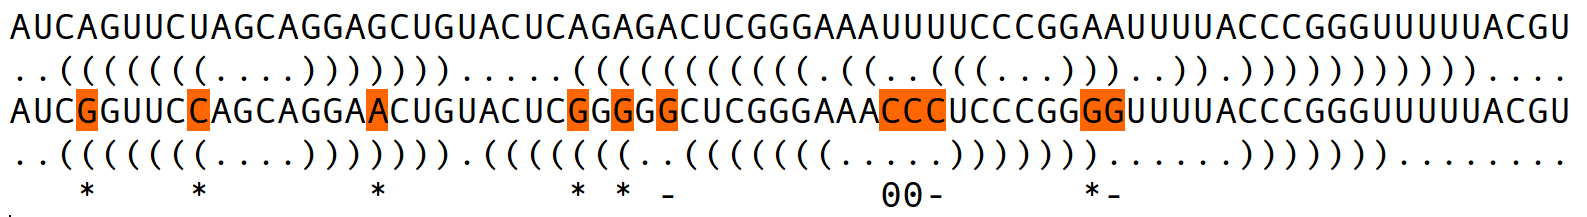
\includegraphics[width = 0.9\textwidth]{figures/mutations.png}
\caption{Seq1 and consensus (seq2) sequence and structure. Mutations are shown in red. The bottom annotation distinguishes mutations in three groups. 1) Those that entail a base pair loss (-). 2) A base pair prevails, even if it's identity is not (*). 3) Mutations in positions with no base pair in either of the structures (0).}
\label{fig:mutations}
\end{figure}




\end{document}
